%\subsection{Schema generale: addestramento degli algoritmi di predizione interno a Grafana con estensioni}
%\begin{figure}[H]
%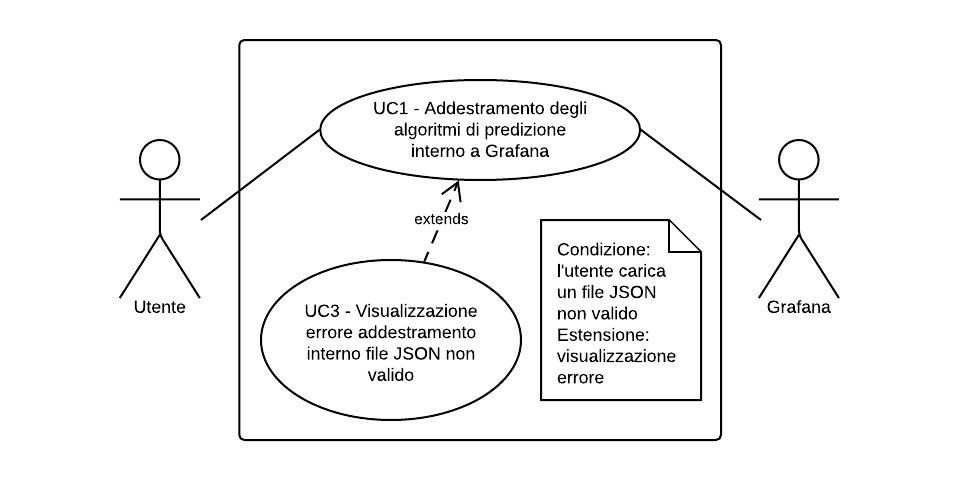
\includegraphics{img/UC1 - Schema generale.png}
%\caption{Schema generale: addestramento degli algoritmi di predizione interno a Grafana con estensioni}
%\end{figure}
\subsection{UC1 - Addestramento degli algoritmi di predizione interno a Grafana}
\begin{figure}[H]
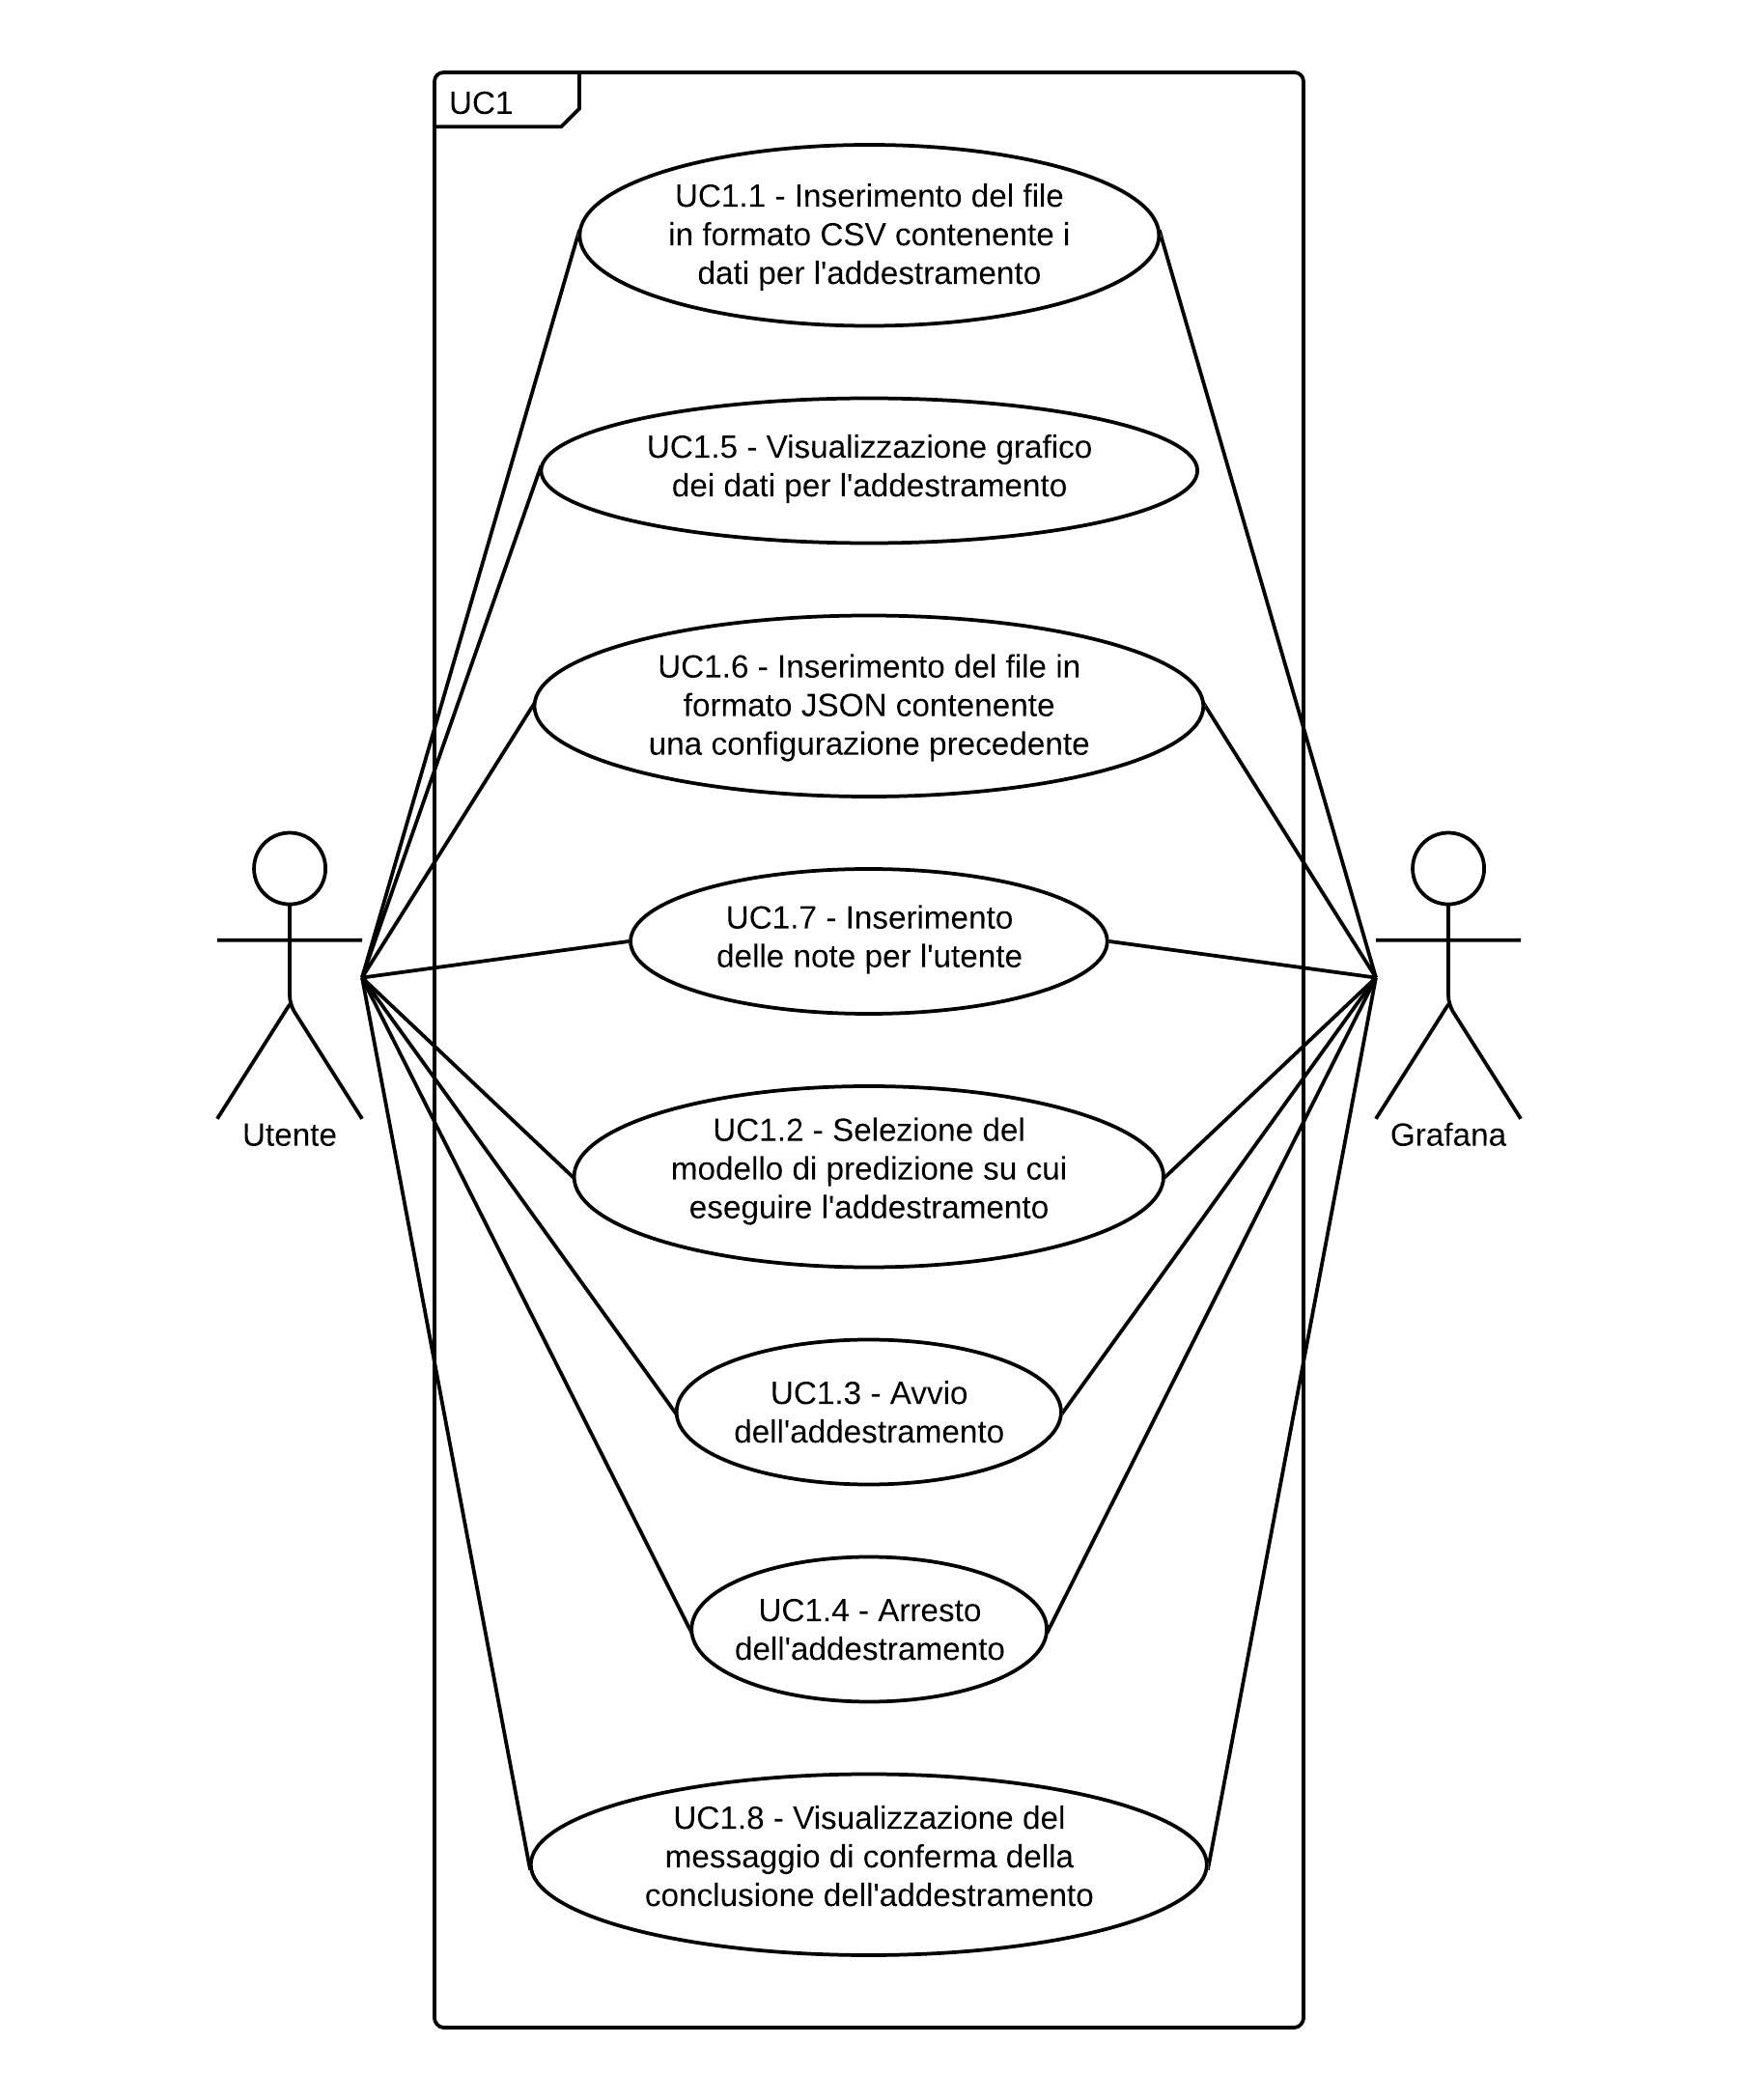
\includegraphics[width=\textwidth,height=\textheight,keepaspectratio]{img/UC1_-_Addestramento_degli_algoritmi_di_predizione_interno_a_Grafana.png}
\caption{Diagramma dello use case UC1}
\end{figure}
\begin{itemize}
	\item \textbf{Codice identificativo}: UC1;
	\item \textbf{Titolo}: addestramento degli algoritmi di predizione interno a Grafana\glo;
	\item \textbf{Attori primari}: utente;
	\item \textbf{Attori secondari}: Grafana\glo;
	\item \textbf{Descrizione}: attività di addestramento degli algoritmi di predizione interna a Grafana\glo, utilizzando dei dati inseriti da un utente autenticato;
	\item \textbf{Precondizioni}: l'utente è autenticato nel sistema software Grafana\glo;
	\item \textbf{Postcondizioni}: Grafana\glosp riceve i dati generati dall'addestramento;
	\item \textbf{Scenario principale}: 
		\begin{enumerate}
			\item inserimento del file in formato CSV contenente i dati per l'addestramento (UC1.1);
			\item visualizzazione grafico dei dati per l'addestramento (UC1.5);
			\item inserimento del file in formato JSON contenente i dati di una configurazione precedente (UC1.6);
			\item inserimento delle note per l'utente (UC1.7);
			\item selezione del modello di predizione su cui eseguire l'addestramento (UC1.2);
			\item avvio dell'addestramento (UC1.3);
			\item arresto dell'addestramento (UC1.4);
			\item visualizzazione del messaggio di conferma della conclusione dell'addestramento (UC1.8).
		\end{enumerate}
	\item \textbf{Estensioni}:
	\begin{itemize}
		\item se il caricamento del file CSV non è avvenuto con successo, viene visualizzato un messaggio di errore (UC17);
		\item se il caricamento del file JSON non è avvenuto con successo, viene visualizzato un messaggio di errore (UC3).
	\end{itemize}
\end{itemize}

\subsubsection{UC1.1 - Inserimento del file in formato CSV contenente i dati per l'addestramento}
\begin{itemize}
	\item \textbf{Codice identificativo}: UC1.1;
	\item \textbf{Titolo}: inserimento del file in formato CSV contenente i dati per l'addestramento;
	\item \textbf{Attori primari}: utente;
	\item \textbf{Attori secondari}: Grafana\glo;
	\item \textbf{Descrizione}: l'utente inserisce nel sistema Grafana\glosp il file in formato CSV che contiene dati per l'addestramento dell'algoritmo di predizione;
	\item \textbf{Precondizioni}: l'utente è autenticato nel sistema software Grafana\glo;
	\item \textbf{Postcondizioni}: il file in formato CSV contenente i dati per l'addestramento è stato inserito correttamente;
	\item \textbf{Scenario principale}: l'utente inserisce il file in formato CSV contenente i dati per l'addestramento.
\end{itemize}
\subsubsection{UC1.5 - Visualizzazione grafico dei dati per l'addestramento}
\begin{itemize}
	\item \textbf{Codice identificativo}: UC1.5;
	\item \textbf{Titolo}: visualizzazione grafico dei dati per l'addestramento;
	\item \textbf{Attori primari}: utente;
	\item \textbf{Descrizione}: l'utente visualizza il grafico a dispersione rappresentante i dati che ha inserito per l'addestramento;
	\item \textbf{Precondizioni}: l'utente è autenticato nel sistema software Grafana\glosp e il file CSV contenente i dati per l'addestramento è stato inserito correttamente;
	\item \textbf{Postcondizioni}: l'utente ha visualizzato il grafico a dispersione rappresentante i dati che ha inserito;
	\item \textbf{Scenario principale}: l'utente visualizza il grafico a dispersione rappresentante i dati che ha inserito.
\end{itemize}
\subsubsection{UC1.6 - Inserimento del file in formato JSON contenente una configurazione precedente}
\begin{itemize}
	\item \textbf{Codice identificativo}: UC1.6;
	\item \textbf{Titolo}: inserimento del file in formato JSON contenente una configurazione precedente;
	\item \textbf{Attori primari}: utente;
	\item \textbf{Attori secondari}: Grafana\glo;
	\item \textbf{Descrizione}: l'utente inserisce nel sistema Grafana\glosp un file JSON che contiene i dati di una configurazione precedente per addestrare nuovamente l'algoritmo di predizione;
	\item \textbf{Precondizioni}: l'utente è autenticato nel sistema software Grafana\glo;
	\item \textbf{Postcondizioni}: il file in formato JSON contenente una configurazione precedente è stato inserito correttamente;
	\item \textbf{Scenario principale}: l'utente inserisce il file in formato JSON contenente una configurazione precedente.
\end{itemize}
\subsubsection{UC1.7 - Inserimento delle note per l'utente}
\begin{itemize}
	\item \textbf{Codice identificativo}: UC1.7;
	\item \textbf{Titolo}: inserimento delle note per l'utente;
	\item \textbf{Attori primari}: utente;
	\item \textbf{Attori secondari}: Grafana\glo;
	\item \textbf{Descrizione}: l'utente inserisce le note che compariranno nel file JSON risultante dall'addestramento dell'algoritmo;
	\item \textbf{Precondizioni}: l'utente è autenticato nel sistema software Grafana\glosp e il file CSV contenente i dati per l'addestramento è stato inserito correttamente;
	\item \textbf{Postcondizioni}: l'utente ha inserito correttamente le note che compariranno nel file JSON risultante dall'addestramento dell'algoritmo;
	\item \textbf{Scenario principale}: l'utente inserisce le note che compariranno nel file JSON risultante dall'addestramento dell'algoritmo.
\end{itemize}
\subsubsection{UC1.2 - Selezione del modello di predizione su cui eseguire l'addestramento}
\begin{itemize}
	\item \textbf{Codice identificativo}: UC1.2;
	\item \textbf{Titolo}: selezione del modello di predizione su cui eseguire l'addestramento;
	\item \textbf{Attori primari}: utente;
	\item \textbf{Attori secondari}: Grafana\glo;
	\item \textbf{Descrizione}: l'utente seleziona il modello di predizione da applicare durante l'addestramento;
	\item \textbf{Precondizioni}: l'utente è autenticato nel sistema software Grafana\glosp e il file CSV contenente i dati per l'addestramento è stato inserito correttamente;
	\item \textbf{Postcondizioni}: l'utente ha selezionato correttamente il modello di predizione;
	\item \textbf{Scenario principale}: l'utente seleziona un modello di predizione per eseguire l'addestramento tra SVM\glosp e RL\glo;
	\item \textbf{Specializzazione}:
	\begin{itemize}
		\item selezione del modello di predizione SVM\glosp (UC1.9);
		\item selezione del modello di predizione RL\glosp (UC1.10).
	\end{itemize}
\end{itemize}
\subsubsection{UC1.9 - Selezione del modello di predizione SVM}
\begin{itemize}
	\item \textbf{Codice identificativo}: UC1.9;
	\item \textbf{Titolo}: selezione del modello di predizione SVM\glo;
	\item \textbf{Attori primari}: utente;
	\item \textbf{Attori secondari}: Grafana\glo;
	\item \textbf{Descrizione}: l'utente seleziona il modello di predizione SVM\glosp da applicare durante l'addestramento;
	\item \textbf{Precondizioni}: l'utente è autenticato nel sistema software Grafana\glosp e il file CSV contenente i dati per l'addestramento è stato inserito correttamente;
	\item \textbf{Postcondizioni}: l'utente ha selezionato SVM\glosp come modello di predizione da applicare;
	\item \textbf{Scenario principale}: l'utente seleziona il modello di predizione SVM\glosp su cui eseguire l'addestramento.
\end{itemize}
\subsubsection{UC1.10 - Selezione del modello di predizione RL}
\begin{itemize}
	\item \textbf{Codice identificativo}: UC1.10;
	\item \textbf{Titolo}: selezione del modello di predizione RL\glo;
	\item \textbf{Attori primari}: utente;
	\item \textbf{Attori secondari}: Grafana\glo;
	\item \textbf{Descrizione}: l'utente seleziona RL\glosp come modello di predizione da applicare durante l'addestramento;
	\item \textbf{Precondizioni}: l'utente è autenticato nel sistema software Grafana\glosp e il file CSV contenente i dati per l'addestramento è stato inserito correttamente;
	\item \textbf{Postcondizioni}: l'utente ha selezionato RL\glosp come modello di predizione da applicare;
	\item \textbf{Scenario principale}: l'utente seleziona il modello di predizione RL\glosp su cui eseguire l'addestramento.
\end{itemize}
\subsubsection{UC1.11 - Selezione del modello di predizione reti neurali}
\begin{itemize}
	\item \textbf{Codice identificativo}: UC1.11;
	\item \textbf{Titolo}: selezione del modello di predizione reti neurali\glo;
	\item \textbf{Attori primari}: utente;
	\item \textbf{Attori secondari}: Grafana\glo;
	\item \textbf{Descrizione}: l'utente seleziona reti neurali\glosp come modello di predizione da applicare durante l'addestramento;
	\item \textbf{Precondizioni}: l'utente è autenticato nel sistema software Grafana\glosp e il file CSV contenente i dati per l'addestramento è stato inserito correttamente;
	\item \textbf{Postcondizioni}: l'utente ha selezionato reti neurali\glosp come modello di predizione da applicare;
	\item \textbf{Scenario principale}: l'utente seleziona il modello di predizione reti neurali\glosp su cui eseguire l'addestramento.
\end{itemize}
\subsubsection{UC1.12 - Selezione del modello di predizione regressioni esponenziali}
\begin{itemize}
	\item \textbf{Codice identificativo}: UC1.12;
	\item \textbf{Titolo}: selezione del modello di predizione regressioni esponenziali;
	\item \textbf{Attori primari}: utente;
	\item \textbf{Attori secondari}: Grafana\glo;
	\item \textbf{Descrizione}: l'utente seleziona regressioni esponenziali come modello di predizione da applicare durante l'addestramento;
	\item \textbf{Precondizioni}: l'utente è autenticato nel sistema software Grafana\glosp e il file contenente i dati per l'addestramento è stato inserito correttamente;
	\item \textbf{Postcondizioni}: l'utente ha selezionato regressioni esponenziali come modello di predizione da applicare;
	\item \textbf{Scenario principale}: l'utente seleziona il modello di predizione regressioni esponenziali su cui eseguire l'addestramento.
\end{itemize}
\subsubsection{UC1.13 - Selezione del modello di predizione regressioni logaritmiche}
\begin{itemize}
	\item \textbf{Codice identificativo}: UC1.13;
	\item \textbf{Titolo}: selezione del modello di predizione regressioni logaritmiche;
	\item \textbf{Attori primari}: utente;
	\item \textbf{Attori secondari}: Grafana\glo;
	\item \textbf{Descrizione}: l'utente seleziona regressioni logaritmiche come modello di predizione da applicare durante l'addestramento;
	\item \textbf{Precondizioni}: l'utente è autenticato nel sistema software Grafana\glosp e il file CSV contenente i dati per l'addestramento è stato inserito correttamente;
	\item \textbf{Postcondizioni}: l'utente ha selezionato regressioni logaritmiche come modello di predizione da applicare;
	\item \textbf{Scenario principale}: l'utente seleziona il modello di predizione regressioni logaritmiche su cui eseguire l'addestramento.
\end{itemize}
\subsubsection{UC1.14 - Selezione del modello di predizione SVM adattata alla Regressione}
\begin{itemize}
	\item \textbf{Codice identificativo}: UC1.14;
	\item \textbf{Titolo}: selezione del modello di predizione SVM\glosp adattata alla Regressione;
	\item \textbf{Attori primari}: utente;
	\item \textbf{Attori secondari}: Grafana\glo;
	\item \textbf{Descrizione}: l'utente seleziona SVM\glosp adattata alla Regressione come modello di predizione da applicare durante l'addestramento;
	\item \textbf{Precondizioni}: l'utente è autenticato nel sistema software Grafana\glosp e il file CSV contenente i dati per l'addestramento è stato inserito correttamente;
	\item \textbf{Postcondizioni}: l'utente ha selezionato SVM\glosp adattata alla Regressione come modello di predizione da applicare;
	\item \textbf{Scenario principale}: l'utente seleziona il modello di predizione SVM\glosp adattata alla Regressione su cui eseguire l'addestramento.
\end{itemize}
\subsubsection{UC1.3 - Avvio dell'addestramento}
\begin{itemize}
	\item \textbf{Codice identificativo}: UC1.3;
	\item \textbf{Titolo}: avvio dell'addestramento;
	\item \textbf{Attori primari}: utente;
	\item \textbf{Attori secondari}: Grafana\glo;
	\item \textbf{Descrizione}: l'utente avvia l'addestramento dell'algoritmo di predizione;
	\item \textbf{Precondizioni}: il file CSV è stato inserito correttamente e il modello di predizione è stato selezionato;
	\item \textbf{Postcondizioni}: l'addestramento è stato avviato con successo;
	\item \textbf{Scenario principale}: l'utente avvia l'addestramento.
\end{itemize}

\subsubsection{UC1.4 - Arresto dell'addestramento}
\begin{itemize}
	\item \textbf{Codice identificativo}: UC1.4;
	\item \textbf{Titolo}: arresto dell'addestramento;
	\item \textbf{Attori primari}: utente;
	\item \textbf{Attori secondari}: Grafana\glo;
	\item \textbf{Descrizione}: l'utente arresta l'addestramento prima della sua normale conclusione;
	\item \textbf{Precondizioni}: l'addestramento è stato avviato con successo;
	\item \textbf{Postcondizioni}: l'addestramento è stato arrestato con successo;
	\item \textbf{Scenario principale}: l'utente arresta forzatamente l'addestramento.
\end{itemize}

\subsubsection{UC1.8 - Visualizzazione del messaggio di conferma della conclusione dell'addestramento}
\begin{itemize}
	\item \textbf{Codice identificativo}: UC1.8;
	\item \textbf{Titolo}: visualizzazione del messaggio di conferma della conclusione dell'addestramento;
	\item \textbf{Attori primari}: utente;
	\item \textbf{Attori secondari}: Grafana\glo;
	\item \textbf{Descrizione}: l'utente visualizza un messaggio di conferma che l'addestramento è stato concluso ed eseguito correttamente;
	\item \textbf{Precondizioni}: l'addestramento è stato concluso con successo secondo il suo normale flusso di esecuzione;
	\item \textbf{Postcondizioni}: l'utente ha visualizzato un messaggio di conferma che l'addestramento è stato concluso ed eseguito correttamente;
	\item \textbf{Scenario principale}: l'utente visualizza un messaggio di conferma che l'addestramento è stato concluso ed eseguito correttamente.
\end{itemize}
